\chapter{System Design}
\section{Database}
For vertex we have chosen to work with a MySQL database. This was ultimately a big decision as we could have gone with any assortment of SQL style databases, a no-SQL database, or could have gone with a graph database, or possibly even a document store.

\subsection{Schemas}
\subsubsection{User Schema}
Something about user schema...
See Figure ~\ref{image:userSchema}

\subsubsection{Channel Schema}
Something about channel schema...
See Figure ~\ref{image:channelSchema}

\subsubsection{Message Schema}
Something about message schema...
See Figure ~\ref{image:messageSchema}

\subsubsection{Session Schema}
Something about session schema...
See Figure ~\ref{image:sessionSchema}

\subsubsection{Member Schema}
Something about member schema...
See Figure ~\ref{image:memberSchema}

\begin{figure}[h!]
    \caption{User Schema}
    \label{image:userSchema}
    \centering
    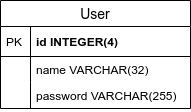
\includegraphics[width=0.3\textwidth]{images/UserSchema.png}
\end{figure}

\begin{figure}[h!]
    \caption{Channel Schema}
    \label{image:channelSchema}
    \centering
    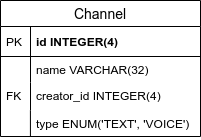
\includegraphics[width=0.3\textwidth]{images/ChannelSchema.png}
\end{figure}

\begin{figure}[h!]
    \caption{Message Schema}
    \label{image:messageSchema}
    \centering
    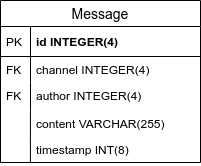
\includegraphics[width=0.3\textwidth]{images/MessageSchema.png}
\end{figure}

\begin{figure}[h!]
    \caption{Session Schema}
    \label{image:sessionSchema}
    \centering
    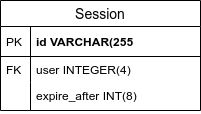
\includegraphics[width=0.3\textwidth]{images/SessionSchema.png}
\end{figure}

\begin{figure}[h!]
    \caption{Member Schema}
    \label{image:memberSchema}
    \centering
    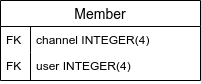
\includegraphics[width=0.3\textwidth]{images/MemberSchema.png}
\end{figure}

\begin{figure}[h!]
    \caption{Database Schema}
    \label{image:databaseSchema}
    \centering
    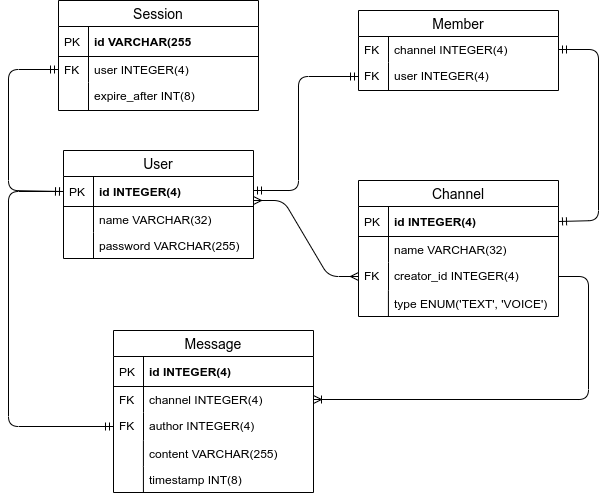
\includegraphics[width=1\textwidth]{images/FullSchemaDesign.png}
\end{figure}